\documentclass{article}
\usepackage{helvet}
\usepackage{graphicx}
\usepackage[margin=1in]{geometry}
\renewcommand{\familydefault}{\sfdefault}
\usepackage{xeCJK}

\setCJKmainfont{Noto Serif CJK TC}
\author{Andr\'es Ponce(0616110)\\
\and
彭思安
}
\title{Introduction To Artificial Intelligence Homework Three Report}

\begin{document}
\maketitle
\section{Background}
For the second assignment of the course, we were tasked to model the game of Minesweeper as a 
constraint satisfiability problem, and apply suitable algorithms to solve a board given an initial 
setup. For the third homework assignment, instead of viewing it in terms of constraints, we model it
as a problem of logical inference. Each cell in our board is then treated as a logical proposition
which can either be true(``safe") or false(``mined").

Given this new approach, the task involved finding an assignment of the nodes which lead to a solved 
board in the end. Thus we treat a set of literals (or their complements) as a \textit{clause}, which
we can compare to other clauses to deduce their truth values. While this is not the most efficient
way to solve a Minesweeper board, it does provide a useful insight into the area of logical satisfiability
as applied to game-playing agents.

\section{Program}
The program is organized in a player module and a board module. The board module contains the information 
contained in every cell, the hint values and the types of the cells. The board module is just a container
for the array containing the nodes.

We also maintain a clause class which, we use to store a list of nodes and their status. This is the main
data structure we check when we want to compare the states two different cells. When the program starts, 
we initially insert the nodes marked as ``safe", which are chosen at random from the board. There are
then other considerations we make when mathing clauses or generating clauses from hints.

The player module is the one playing the game. This module is repsonsible for maintaining the knowledge
base of the unassigned and the nodes whose status we have already determined. To do the matching, we 
try to match the node that is being checked with the other clauses that we have in our knowledge base.

The issues in this assignment come from the complexity of matching different propositions composed of nodes in our board. This introduced an extra layer of
complexity at the moment checking a valid move. We have to match nodes based on 
interpreting them as logical propositions, which is not the most intuitive way
of looking at a problem.

The main function takes a look at whether the board requirements are fulfilled, so we 
check if our board is actually completed. After that, we take different actions based 
on if the node we are checking is a single literal or not. If it is, we apply the 
pairwise matching proces with all the other elements in our knowledge base. When in this
process, we generate new clauses and add them to our knowledge base to check later. 
Only if it is a safe cell do we query the board for the hints at that spot.

This approach to solving the board is more complicated than constrain satisfaction 
approach from the previous assignment. Thus, it was quite hard to even think of how 
to generate clauses from hints, even given the help in the \texttt{.pdf} file.

The player and the board module are only iteracting to query, all the logic occurs in the player module.
\section{Further Discussion}
	\subsection{How could we use first-order logic here?}
		First order logic differs from propositional logic in its power at expressing propositions. For 
		example, a sentence such as ``Every student will get a perfect score on this homework assignment"
		cannot be easily written using only propositional logic, unless we number all $n$  students  in the
		class and say the he or she will get a perfect score; something like 
		$p_{1}\land p_{2}\land ...\land p_{n}$.
		
		First order logic allows us to use universal or existential \textit{quantifiers} which make a 
		proposition apply to all the elements in the specified domain. Thus, if $g(x)$ represents the 
		proposition ``x will receive a perfect score on this assignment", we could model the previous
		sentence as $\forall x g(x)$, where x are the students in the course.
	
		Since first-order logic already deals with applying predicate symbols to constant symbols,
		applying this structure to that of a program might prove more straightforward than using 
		propositional logic. We could apply some functions to check the relations between the different
		objects. If we choose appropriate relations to check, maybe such to check a valid assignment 
		or the number of adjacent objects, may be a more intuitive approach to this problem.
	\subsection{Is forward chaining or backward chaining applicable to this problem?}
		Yes, there are ways we could use chaining in this problem. To arrive at a conclusion $c$, we could recursively check all the propositions whose values
		we can infer. Special attention would be gven to inferring the value of 
		the literals is $c$'s premises. Backward chaining might be harder to implement
		since we would already need a solution to implement before inferring the 
		values of its premises.

		For forward chaining, the recursion tree would eventually encompass all the 
		values that can be reached if we recurse. Once we build the tree, we could 
		merely query the truth value of a literal whenever we required it. Thus 
		recursively inferring values might prove a possible way to utilize forward 
		chaining.
	\subsection{How could we imporve the success rate of ``guessing" when you want to proceed from a
			``stuck" game.}
		Currently, we are only guessing that we are stuck when we do not make any moves for a couple
		turns. However, if we analyze the conditions on which the games get stuck, we could be able
		to perform a check every time we select a clause or every time we mark a node. This way, 
		if we are not going anywhere, we could detect a stuck game before spending several turns
		without making any moves.

	\subsection{How could we modify the method of Assignment 2 to solve the current problem?}
		We could modify the main algorithm from Assignment 2 to work in this assignment. For assignment
		2, after checking if the board is solved, we checked if assigning the node to be a mine was a 
		valid assignment based on the checking the adjacent nodes. In this assignment, we could attempt
		to select nodes and instead of checking its constraints, we could match it with our knowledge base
		to derive it's truth value. If we can do this for the current node, we can safely recurse on the
		adjacent nodes. If we cannot clearly match the node, we attempt to assign TRUE and FALSE to the 
		current node and see which assignment leads to a solved board.

		An approach resembling the above would still carry the same structure as the previous assignment,
		while using the techniques learned in this assignment involving propositional logic.
\section{Code Images}
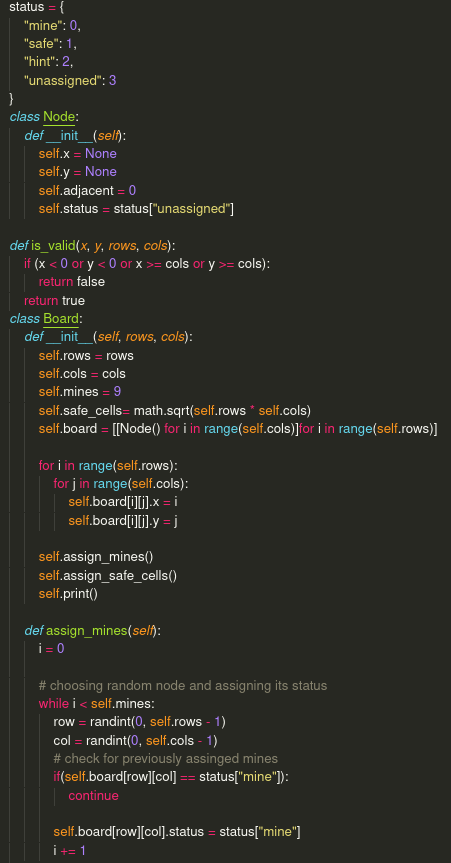
\includegraphics[scale=0.5]{s1.png}

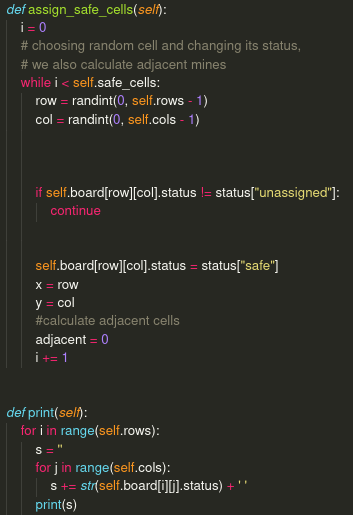
\includegraphics[scale=0.5]{s2.png}

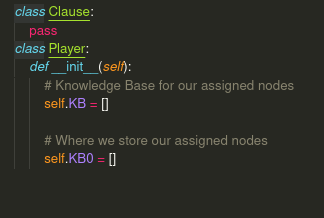
\includegraphics[scale=0.5]{s3.png}

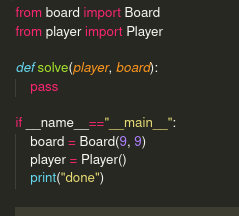
\includegraphics[scale=0.5]{s4.png}
\end{document}
